\section{Reviewer 2}

\subsection{Question 1}
\begin{reviewcomment}
Clarify measured vs. simulated and validate the model. State whether each baseline is real hardware or gem5, and validate FluxArch against a fabricated reference---the headline 6.83$\times$/9.84$\times$ claims depend on this.
\end{reviewcomment}
We sincerely thank you for your helpful and constructive suggestion. We agree that the evaluation must distinguish native measurements from simulation and provide direct evidence for the modeled components.

\begin{enumerate}[label=(\arabic*)]
\setlength{\emergencystretch}{1em}
\item \textbf{Measured versus simulated results.} The Intel, AMD, FT, A100, and H100 baselines are executed and measured on native hardware, whereas \name\ performance is simulated in gem5 and its package power and area are modeled with McPAT and CACTI. We revised the platform description so that the measurement and modeling boundary is explicit for every platform. The native results are hardware measurements, while the \name\ results are calibrated simulation estimates.


\revisionlocation{The distinction between native measurements and modeled results is clarified in \textbf{Section 6.1}.

The platform-specific evaluation and power-accounting methods are specified in \textbf{Table~5}, replacing original \textbf{Table~3}. Panel (a) revises the platform specifications, while panel (b) adds the evaluation methods and power-accounting boundaries.}

\par\noindent\begin{minipage}{\linewidth}
\excerptlabel{Original (Table~3, page 14):}\par
% Original manuscript: Table 3
\begin{figure}[H]
  \centering
  \fbox{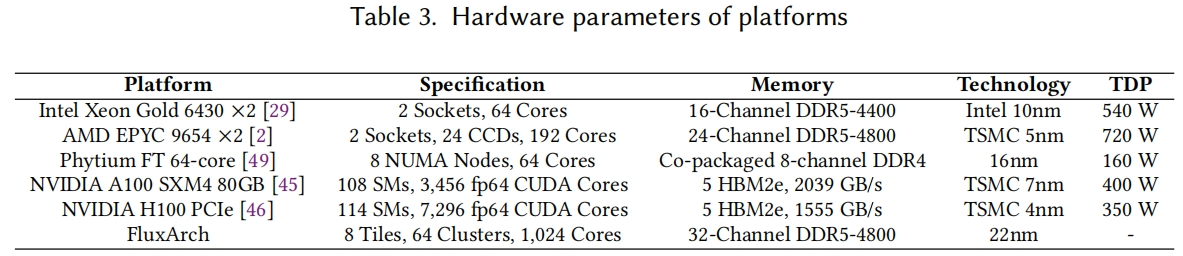
\includegraphics[width=0.9\textwidth]{figures/O-tab3.png}}
\end{figure}
\end{minipage}\par\medskip

\par\noindent\begin{minipage}{\linewidth}
\excerptlabel{Revised (Table~5, page 15):}\par
% Revised manuscript: Table 5
\begin{figure}[H]
  \centering
  \fbox{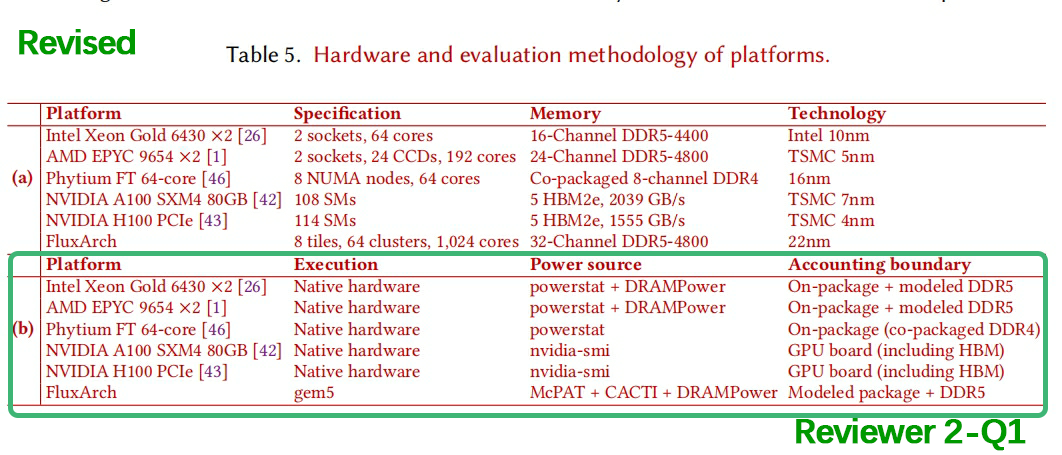
\includegraphics[width=0.9\textwidth]{news/R2-Q1-tab5.png}}
\end{figure}
\end{minipage}\par\medskip

\item \textbf{Model validation.} We added six controlled comparisons against RK3562 Cortex-A53 silicon for the core and cache/DRAM paths and derived Engine latency directly from fixed-latency RTL operators and loop bounds. The silicon comparison yields matching checksums, 6.7\% mean absolute percentage error, and 13.5\% maximum absolute percentage error; the Engine expression is derived from the implementation. This establishes implementation traceability, not an independent statistical calibration between two timing models. We describe these results as calibrated simulation evidence while clearly retaining the limitation that the complete 1,024-core system has not been fabricated.

\revisionlocation{The deterministic Engine latency is derived from RTL operator timing and loop bounds in \textbf{Section 4.2}.}

\par\noindent\begin{minipage}{\linewidth}
\excerptlabel{Figure~9 (page 9):}\par
% Manuscript: Figure 9
\begin{figure}[H]
  \centering
  \fbox{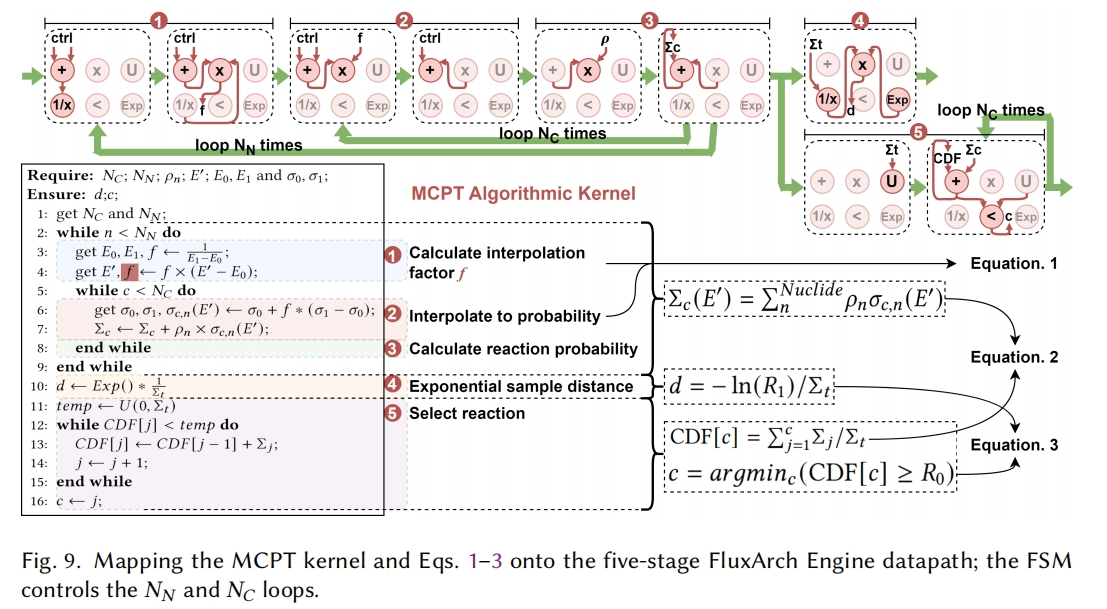
\includegraphics[width=0.9\textwidth]{figures/fig9.png}}
\end{figure}
\end{minipage}\par\medskip

\excerptlabel{Added (Section 4.2, pages 9--10):}\par
\begin{manuscriptexcerpt}
\redsentence{Here, $N_N$ denotes the number of nuclides and $N_C$ the number of reaction channels per nuclide; they determine the outer and inner loop bounds, respectively.}

\redsentence{\textbf{Deterministic Timing Model.}} \redsentence{To meet the timing requirements at the same target clock frequency as the \name\ Core, the RTL operators are partitioned into different numbers of pipeline stages.} \redsentence{Table~2(b) lists the fixed RTL operator latencies using the same symbols as Fig.~9.} \redsentence{Under the computation-only boundary used by the Engine model---excluding launch, stage-transition, \texttt{out\_valid}, and CPU/MMIO input-wait cycles---the five stages take 10 cycles for \redone~($+\to1/x\to\times$, $3+4+3$), 12 cycles for \redtwo~and \redthree~combined~($+\to\times\to+\to\times$, $3+3+3+3$), 7 cycles for \redfour~($1/x\to\times$, $4+3$), and $3+4N_C$ cycles for \redfive~($U\to\{+\to<\}^{N_C}$, $3+N_C(3+1)$).} \redsentence{The resulting latency is
\[
\begin{array}{rl}
L_{\mathrm{Engine}}(N_N,N_C)
&=N_N(10+12N_C)+\max(7,3+4N_C) \\
&=12N_NN_C+10N_N+4N_C+3.
\end{array}
\]} \redsentence{It depends only on the programmed nuclide and reaction-channel counts, not on the numerical operand values.} \redsentence{The gem5 Engine timing directly implements this RTL-derived expression rather than an empirically fitted latency.}
\end{manuscriptexcerpt}



\par\noindent\begin{minipage}{\linewidth}
\revisionlocation{The operator latencies and five-stage timing parameters supporting this derivation are added in \textbf{Table~2(b)}.}

\excerptlabel{Added (Table~2(b), page 10):}\par
% Revised manuscript: Table 2(b)
\begin{figure}[H]
  \centering
  \fbox{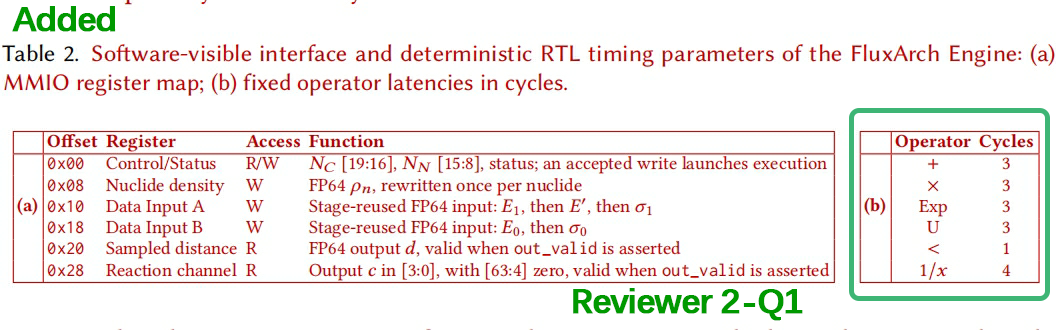
\includegraphics[width=0.9\textwidth]{news/R2-Q1-tab2b.png}}
\end{figure}
\end{minipage}\par\medskip


\revisionlocation{The matched silicon/simulation calibration protocol, errors, and validation scope are described in \textbf{Section 6.1}.}

\excerptlabel{Added (Section 6.1, page 13):}\par
\begin{manuscriptexcerpt}
\redsentence{\textbf{Core Timing Calibration.}} \redsentence{We calibrate the 2-GHz in-order \name\ Core model against a 2-GB KickPi K3B with a 22-nm quad-core RK3562 Cortex-A53~\papercite{kickpi-k3b,rockchip-rk3562}.} \redsentence{The native process is pinned to one 2-GHz core under stable thermal conditions; both platforms use identical source, GCC 13.3, \texttt{-O2 -fno-tree-vectorize}, seed, warm-up, and timed region.} \redsentence{All six checksums match.} \redsentence{Table~3 reports latency and signed error $100(T_{\rm gem5}-T_{\rm K3B})/T_{\rm K3B}$; across the six tests, the mean and maximum absolute percentage errors are 6.7\% and 13.5\%, respectively.} \redsentence{FluxArch's absolute throughput and speedups are obtained directly from the calibrated simulations.}

\redsentence{This silicon comparison calibrates the core and cache/DRAM paths, not the complete 1,024-core hierarchy.} \redsentence{Section~4.2 establishes RTL-to-gem5 Engine timing traceability, and Sections~6.5--6.7 evaluate the modeled full system; we therefore report calibrated simulation evidence, not fabricated-system measurements.}
\end{manuscriptexcerpt}
\begin{excerptreferences}
\paperreference{rockchip-rk3562}
\paperreference{kickpi-k3b}
\end{excerptreferences}

\par\noindent\begin{minipage}{\linewidth}
\revisionlocation{The six RK3562 calibration cases and measured-versus-simulated latencies are added in \textbf{Table~3}.}

\excerptlabel{Added (Table~3, page 13):}\par
% Revised manuscript: Table 3
\begin{figure}[H]
  \centering
  \fbox{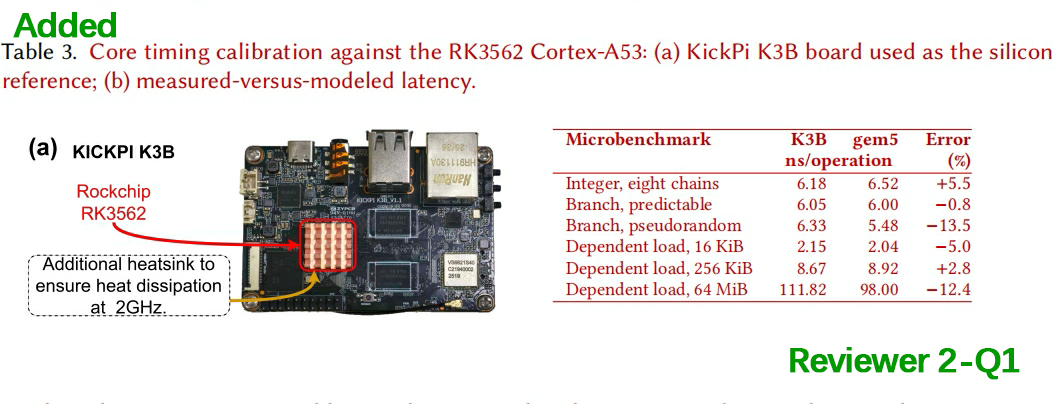
\includegraphics[width=0.9\textwidth]{news/R2-Q1-tab3.png}}
\end{figure}
\end{minipage}\par\medskip


\end{enumerate}

\subsection{Question 2}
\begin{reviewcomment}
Resolve the L2-residency contradiction. Quantify per benchmark whether the replicated database fits in the 4 MB L2 (esp. XSBench); this conflicts with Fig. 3(e) and underpins the speedups.
\end{reviewcomment}
Our performance evaluation does not assume that the benchmark databases reside entirely in L2. The gem5 cache model accounts for finite cache capacity, cache-line replacement, and accesses to the memory hierarchy following L2 misses. The reported throughput therefore reflects capacity-limited caching and the effects of the configured replacement policy, rather than idealized all-hit behavior. For XSBench, the 64.58\% L2 read hit rate and 617.79 bytes of DRAM reads per lookup in Table~6(a) explicitly demonstrate that substantial off-chip accesses remain.

The capacity evidence in Fig.~3(d,e) is consistent with this evaluation. Fig.~3(d) lists a 241~MB complete database and a 62~MB energy-dense working set even for the Small configuration, both exceeding the 4~MB cluster-local L2. These sizes explain the cache-overflow schematic in Fig.~3(e): neither the complete database nor the energy-dense working set can fit in L2. However, capacity overflow does not preclude caching and reusing a subset of lines.

We revised the description of LLC-aware mapping to clarify that the strategy benefits from partial data reuse within each cluster's shared L2 and does not require the entire benchmark database to fit in its 4 MiB capacity. To support this clarification, we added per-workload database size, L2 hit rate, and normalized DRAM traffic. The Quicksilver databases occupy only 0.055--0.318 MiB, whereas the 241-MiB XSBench database is approximately $60.25\times$ the L2 capacity; XSBench therefore cannot reside in L2, although its shared read-only accesses still obtain partial temporal reuse.

\revisionlocation{The full-residency implication is corrected in \textbf{Section 5.2} and \textbf{Figure 3}, which now describes capacity-limited reuse within the shared L2.}

\par\noindent\begin{minipage}{\linewidth}
\excerptlabel{Figure~3 (page 5):}\par
% Manuscript: Figure 3
\begin{figure}[H]
  \centering
  \fbox{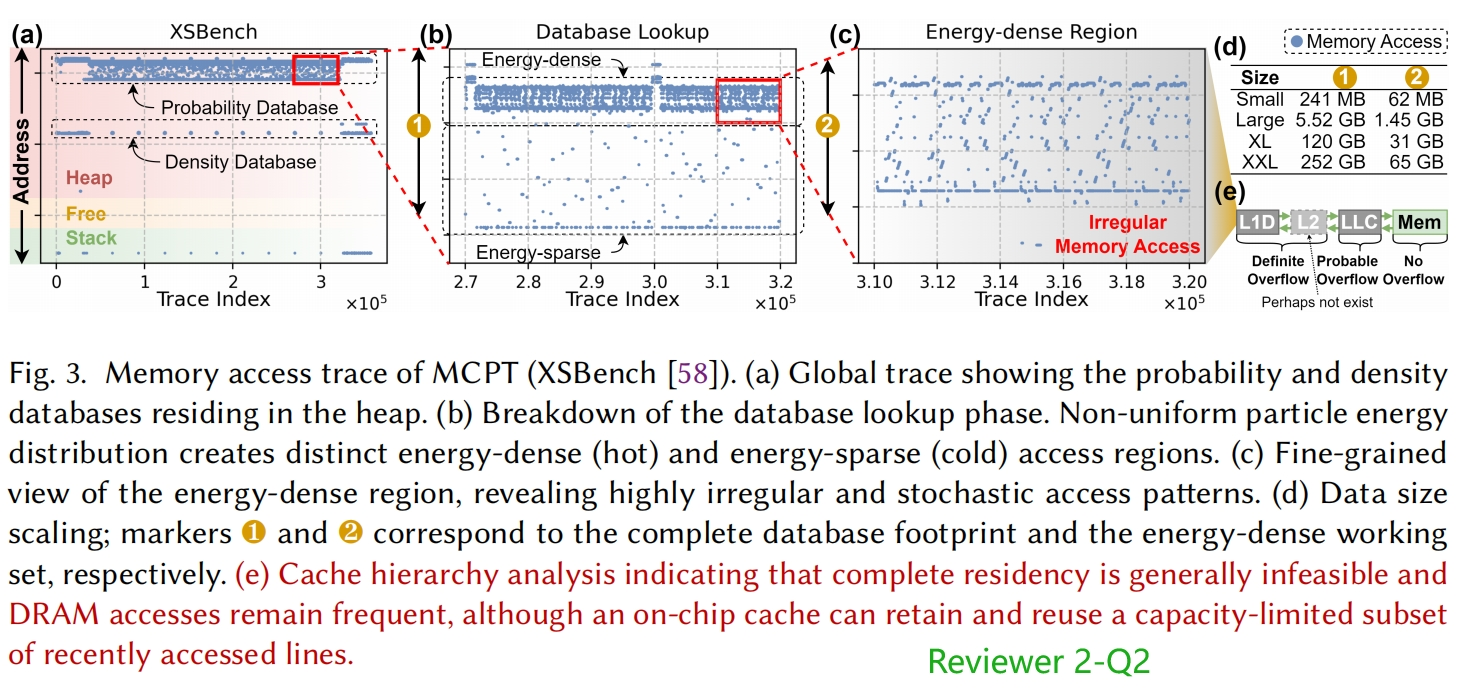
\includegraphics[width=0.9\textwidth]{figures/fig3.png}}
\end{figure}
\end{minipage}\par\medskip

\excerptlabel{Original (Section 5.2, page 12):}\par
\begin{manuscriptexcerpt}
\graysentence{Locality-Optimized Data Replication: The hybrid model treats each process as an isolated memory domain, allowing us to replicate read-only density database and other shared data into local memory.} \graysentence{Provided the dataset fits within the LLC, this converts memory-bound irregular lookups into low-latency L2 cache hits, bypassing the DRAM bottleneck.}
\end{manuscriptexcerpt}


\excerptlabel{Revised (Section 5.2, pages 11--12):}\par
\begin{manuscriptexcerpt}
\redsentence{Shared-Database Reuse within an LLC Domain: Threads belonging to the same MPI process access a common read-mostly physics database.} \redsentence{Binding these threads to cores sharing the cluster-local 4~MB L2 allows a cache line fetched by one thread to be reused by other threads in the process.} \redsentence{This optimization does not require the complete database or working set to reside in L2.} \redsentence{Instead, the shared L2 retains a capacity-limited subset of recently accessed cache lines, reducing rather than eliminating DRAM accesses.} \redsentence{Each process places its database replica in its local NUMA memory domain, avoiding remote-memory accesses when an L2 miss occurs.}
\end{manuscriptexcerpt}

\revisionlocation{The workload-dependent L2 residency and DRAM traffic are analyzed in \textbf{Section 6.5}.}

\excerptlabel{Added (Section 6.5, pages 17--18):}\par
\begin{manuscriptexcerpt}
\redsentence{Table~6(a) clarifies that the affinity strategy does not rely on universal database residency in the 4~MB cluster-local L2.} \redsentence{The databases of CORAL2-P1, CORAL2-P2, CTS2 and Homogeneous occupy only 0.055--0.318~MiB per process and achieve 91.98\%--95.81\% L2 read hit rates.} \redsentence{In contrast, the 241~MiB XSBench database is approximately 60$\times$ the L2 capacity.} \redsentence{Nevertheless, its 64.58\% L2 read hit rate shows that the cache retains a useful capacity-limited subset, while the remaining misses generate 617.79 bytes of DRAM reads per lookup.} \redsentence{For Quicksilver, DRAM traffic is normalized per transported segment; for XSBench, it is normalized per cross-section lookup.} \redsentence{These measurements are consistent with the intended mechanism: the shared L2 captures partial reuse but neither requires complete working-set residency nor eliminates DRAM traffic.}
\end{manuscriptexcerpt}

\par\noindent\begin{minipage}{\linewidth}
\revisionlocation{The database sizes, L2 hit rates, and normalized DRAM traffic are added in \textbf{Table~6(a)}.}

\excerptlabel{Added (Table~6(a), page 18):}\par
% Revised manuscript: Table 6(a)
\begin{figure}[H]
  \centering
  \fbox{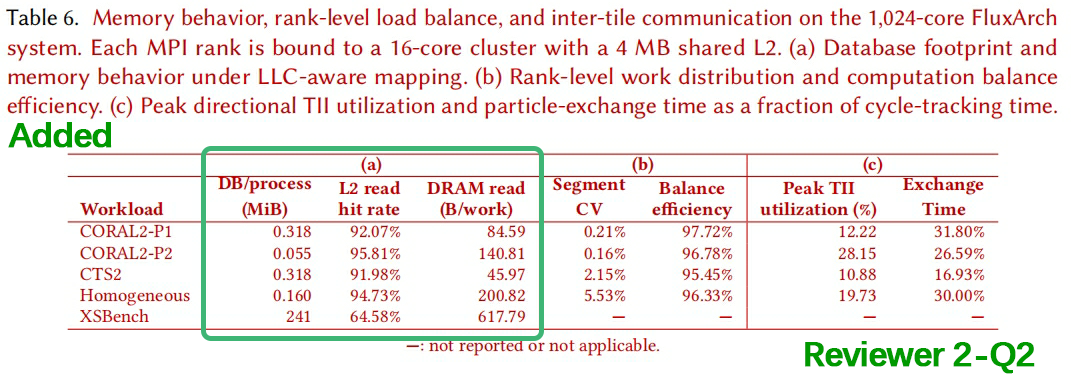
\includegraphics[width=0.9\textwidth]{news/R2-Q2-tab6a.png}}
\end{figure}
\end{minipage}\par\medskip

\subsection{Question 3}

\begin{reviewcomment}
Report DRAM-inclusive energy, or justify why excluding off-chip DRAM does not bias a memory-bound workload.
\end{reviewcomment}

We agree that excluding DRAM would bias the system-level energy comparison for these memory-intensive workloads. We changed the evaluation to include co-packaged DDR4/HBM through device telemetry and off-package DDR5 through the same traffic-based DRAMPower methodology, and we vary the modeled DDR5 component over a $0.5\times$--$2\times$ range to assess sensitivity. The conservative process-scaled geometric-mean DRAM-inclusive energy-efficiency advantage remains 1.77$\times$ over H100 and 6.65$\times$ over Intel.

We now explain the choice of the $0.5\times$--$2\times$ range in \textbf{Section 6.1}. Ghose et al.~\papercite{ghose2018vampire} measured DDR3L read currents averaging 54.1\% below datasheet values for one vendor and data-pattern-dependent read-power differences of up to 91.6\%. Shi et al.~\papercite{shi2025drampower} report that DDR4 calibration reduced DRAMPower energy estimates by roughly half for most evaluated SPEC2006 workloads. These results motivate testing sizable modeling discrepancies, but do not establish an error bound for our DDR5 configuration. We therefore select reciprocal factors of 0.5 and 2 to test both overestimation and underestimation, with package power fixed; the range is a sensitivity-analysis choice, not a statistical confidence interval.

For process-scaled energy-efficiency bounds, we independently vary only the scaled FluxArch package power by $\pm30\%$ and each modeled off-package DRAM component over $0.5\times$--$2\times$, while keeping throughput and measured baseline package power fixed. We recompute the performance/W ratio at every endpoint combination and report its minimum and maximum; external DRAM power is not subject to process-node scaling or its 30\% margin.

\begin{excerptreferences}
\paperreference{ghose2018vampire}
\paperreference{shi2025drampower}
\end{excerptreferences}

\revisionlocation{The common DRAM-power accounting model and sensitivity bounds are specified in \textbf{Section 6.1}.

The DRAM-inclusive energy-efficiency results and conservative lower bounds are updated in \textbf{Section 6.2}.}

\excerptlabel{Original (Section 6.2, pages 14--15):}\par
\begin{manuscriptexcerpt}
\graysentence{\textbf{Iso-Process Energy Efficiency}.} \graysentence{As shown in Fig.~13(b), the energy efficiency advantage is even more pronounced.} \graysentence{By comparing projected iso-process nodes, we isolate the architectural contributions.} \graysentence{According to Section. 6.1, the power projection error is 30\%.} \graysentence{Therefore, we incorporate this margin into our energy efficiency evaluation, which is represented as error bars in our results.} \graysentence{Without the workload orchestration, the energy efficiency of \name, mainstream server CPUs and high-end GPUs is at odds with each other.} \graysentence{With the orchestration enabled, optimizing data locality and minimizing cross-tile traffic, \name\ demonstrates a superior geometric mean energy efficiency improvement from \textbf{3.98}$\boldsymbol{\times}$ (vs. \ft, 5.69$\times$ discounted by 30\%) to \textbf{9.84}$\boldsymbol{\times}$ (vs. \intel, 14.06$\times$ discounted by 30\%) even accounting for the potential projection error of pessimistic assumption.} \graysentence{We also report the energy efficiency of the raw, unscaled data based on the 22 nm technology node.} \graysentence{Even in this case, \name\ still achieves an energy efficiency improvement of 1.17$\times$ (vs. \hopper) to 4.59$\times$ (vs. \intel).}
\end{manuscriptexcerpt}

\excerptlabel{Revised (Section 6.2, pages 15--16):}\par
\begin{manuscriptexcerpt}
\redsentence{\textbf{DRAM-Inclusive Energy Efficiency.}} \redsentence{Fig.~13(c,d) reports DRAM-inclusive power and energy efficiency under the sensitivity bounds defined in Section~6.1.} \redsentence{Process-scaled results separate architectural effects from process scaling while accounting consistently for external memory.}

\redsentence{In the process-scaled comparison, \name\ improves geometric-mean DRAM-inclusive efficiency by \textbf{2.85}$\boldsymbol{\times}$ over \hopper\ to \textbf{10.58}$\boldsymbol{\times}$ over \intel.}

\redsentence{The sensitivity analysis preserves the process-scaled conclusion: across the combined DRAM and technology-scaling bounds, the geometric-mean improvement with orchestration remains 1.77$\times$ over \hopper\ and 6.65$\times$ over \intel\ at the conservative lower bound.}
\end{manuscriptexcerpt}

\par\noindent\begin{minipage}{\linewidth}
\revisionlocation{The DRAM-inclusive power breakdown and energy-efficiency results are plotted in revised \textbf{Figure~13(c,d)}. Panel (c) is newly added; panel (d) revises the original energy-efficiency plot.}

\excerptlabel{Original (Figure~13, page 15):}\par
% Original manuscript: Figure 13
\begin{figure}[H]
  \centering
  \fbox{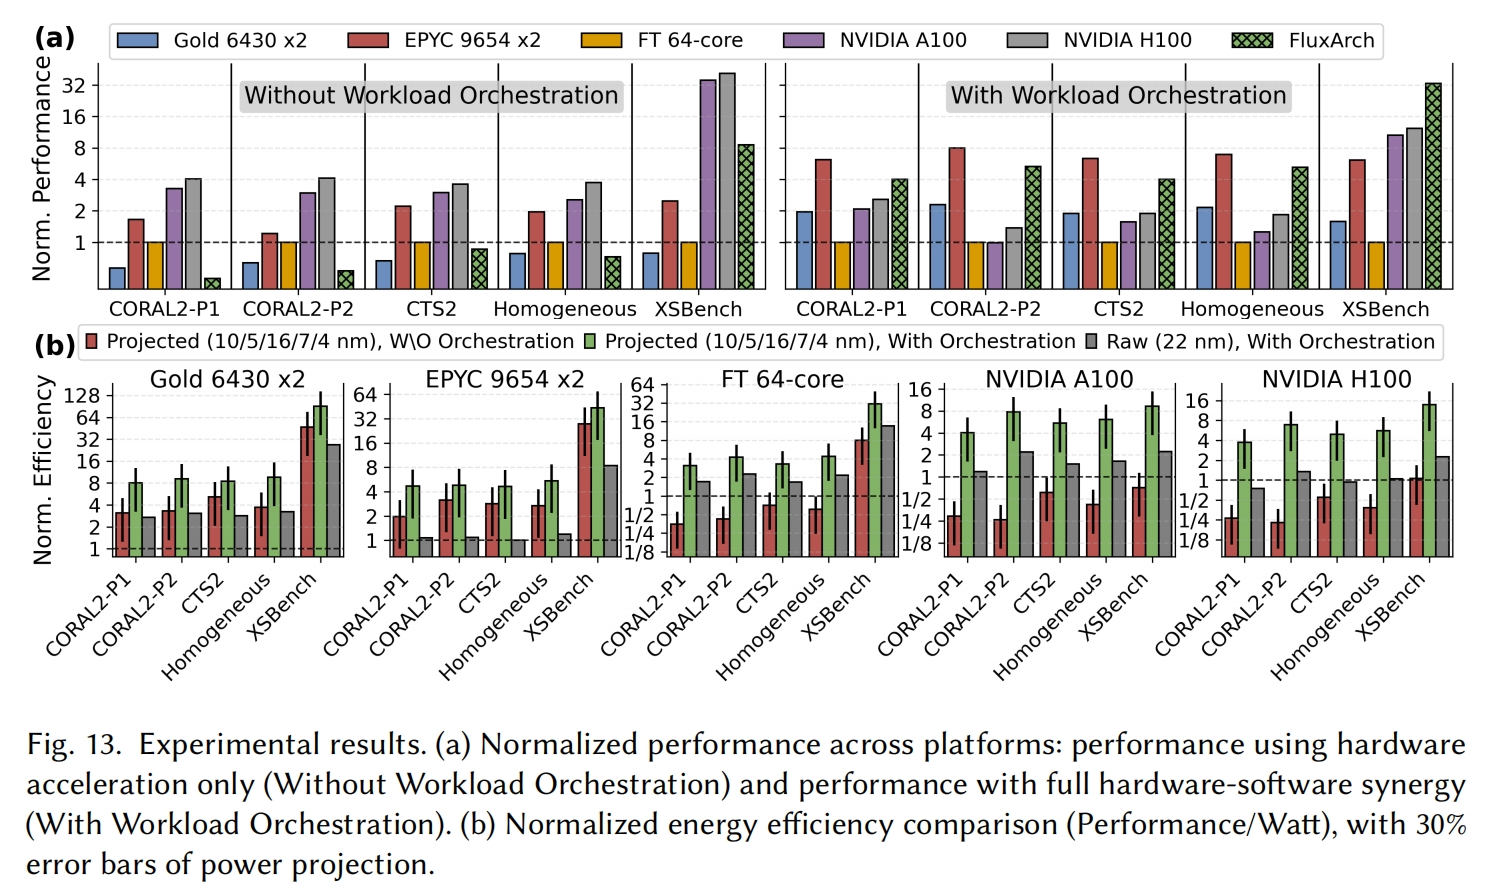
\includegraphics[width=0.9\textwidth]{figures/O-fig13.png}}
\end{figure}
\end{minipage}\par\medskip

\par\noindent\begin{minipage}{\linewidth}
\excerptlabel{Revised (Figure~13, page 16):}\par
% Revised manuscript: Figure 13
\begin{figure}[H]
  \centering
  \fbox{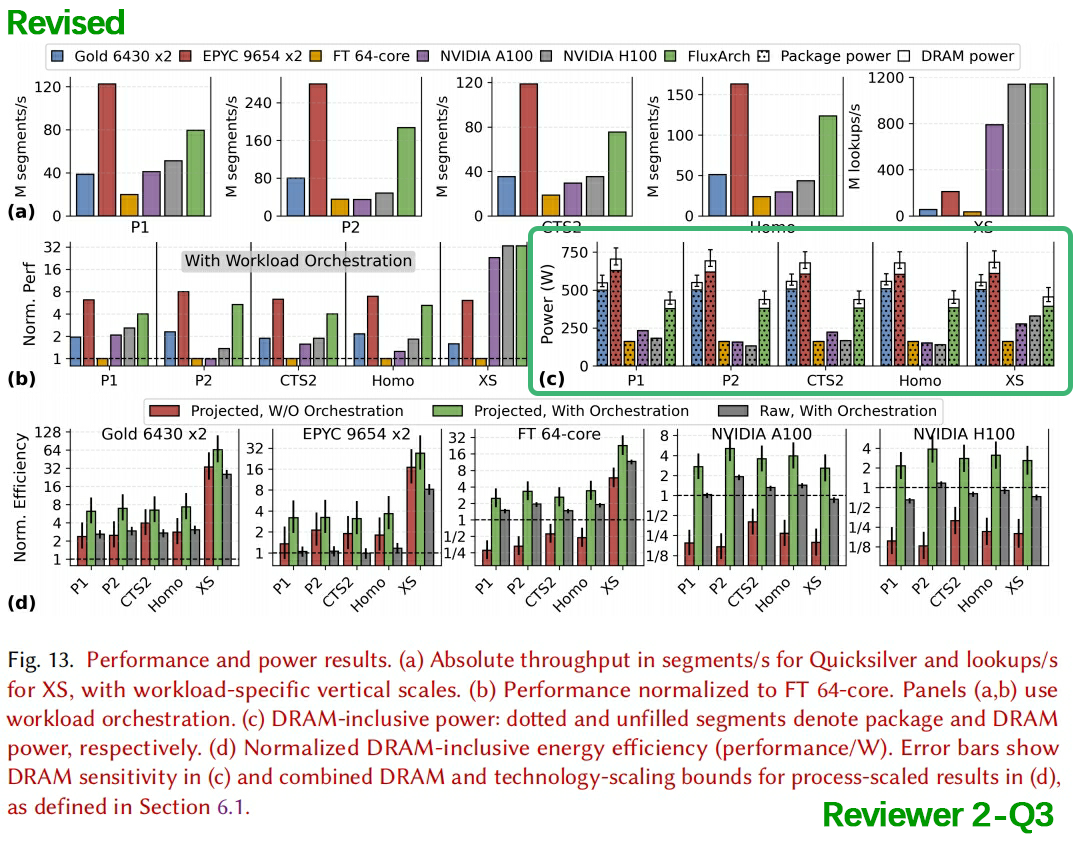
\includegraphics[width=0.9\textwidth]{news/R2-Q3-fig13.png}}
\end{figure}
\end{minipage}\par\medskip

\subsection{Question 4}
\begin{reviewcomment}
Fix inconsistencies and add absolutes. Reconcile the conflicting engine-area and energy figures, report absolute throughput (histories/sec), and do a language pass.
\end{reviewcomment}
We reconciled the Engine-area and energy-efficiency figures, added absolute throughput, and revised the language.

\begin{enumerate}[label=(\arabic*)]
\setlength{\emergencystretch}{1em}
\item \textbf{Engine-area consistency.} The correct synthesized Engine area is 0.270~mm$^2$, compared with 0.763~mm$^2$ for the standard FPU. We corrected the inconsistent value and percentage throughout the manuscript. The consistent result is that the Engine occupies 35.4\% of the FPU area, corresponding to a 64.6\% reduction.

\revisionlocation{The Engine-area value and its comparison with the standard FPU are corrected in \textbf{Section 3.3}.}

\excerptlabel{Original (Section 3.3, page 7):}\par
\begin{manuscriptexcerpt}
\graysentence{To evaluate the area efficiency of architectural specialization, we synthesized both a standard full-functional FPU and our engine using open-source RTL at a 22 nm technology node (as detailed in Section 6.3).} \graysentence{By eliminating the extensive logic required for full FP32/FP64 precision and stripping away general-purpose scheduling, our dedicated engine occupies only 0.251~mm$^2$---a 67\% reduction in footprint compared to a standard FPU (0.763~mm$^2$).} \graysentence{This specialized FP64-only design maximizes computational density per unit area, directly addressing the low arithmetic intensity of general-purpose cores while providing the throughput necessary for large-scale MCPT simulations.}
\end{manuscriptexcerpt}

\excerptlabel{Revised (Section 3.3, page 6):}\par
\begin{manuscriptexcerpt}
\graysentence{To evaluate the area efficiency of architectural specialization, we synthesized both a standard full-functional FPU and our engine using open-source RTL~\papercite{hardfloat} at a 22 nm technology node (as detailed in Section 6.3).} \redsentence{By eliminating the extensive logic required for full FP32/FP64 precision and stripping away general-purpose scheduling, our dedicated engine occupies 0.270~mm$^2$---a 64.6\% reduction in footprint compared with a standard FPU (0.763~mm$^2$).} \graysentence{This specialized FP64-only design maximizes computational density per unit area, directly addressing the low arithmetic intensity of general-purpose cores while providing the throughput necessary for large-scale MCPT simulations.}
\end{manuscriptexcerpt}
\begin{excerptreferences}
\paperreference{hardfloat}
\end{excerptreferences}

\revisionlocation{The area analysis is corrected in \textbf{Section 6.3} to use the same Engine area and reduction percentage.}

\excerptlabel{Original (Section 6.3, page 15):}\par
\begin{manuscriptexcerpt}
\graysentence{The system hierarchy is optimized for high computational density (Fig.~14(c)), with Compute Tiles dominating the design (97\% of total area) and compute cores accounting for approximately 70\% of the entire system's area.} \graysentence{The \name\ Engine, shown in Fig.~14(b), is remarkably area-efficient, occupying only one-third of the footprint of a standard FPU.} \graysentence{This specialization for MCPT achieves higher throughput per mm$^2$ than general-purpose units.} \graysentence{A detailed floorplan of the Engine (Fig.~14(a)) reveals a total area of 0.27~mm$^2$, where FP64 functional units occupy over 97\% of the engine's area.} \graysentence{This extreme functional density is achieved by stripping away single-precision support and complex control logic, dedicating nearly all silicon to the primary computational bottlenecks of MCPT.}
\end{manuscriptexcerpt}

\excerptlabel{Revised (Section 6.3, page 17):}\par
\begin{manuscriptexcerpt}
\graysentence{The system hierarchy is optimized for high computational density (Fig.~14(c)), with Compute Tiles dominating the design (97\% of total area) and compute cores accounting for approximately 70\% of the entire system's area.} \redsentence{The \name\ Engine, shown in Fig.~14(b), is remarkably area-efficient, occupying 0.270~mm$^2$, or 35.4\% of the 0.763~mm$^2$ standard-FPU footprint.} \graysentence{This specialization for MCPT achieves higher throughput per mm$^2$ than general-purpose units.} \redsentence{A detailed floorplan of the Engine (Fig.~14(a)) shows that FP64 functional units occupy over 97\% of the engine area.} \graysentence{This extreme functional density is achieved by stripping away single-precision support and complex control logic, dedicating nearly all silicon to the primary computational bottlenecks of MCPT.}
\end{manuscriptexcerpt}


\item \textbf{Energy-efficiency consistency.} The original manuscript mixed nominal energy-efficiency improvements (5.69$\times$--14.06$\times$ in the Introduction) with conservative values after a 30\% discount (3.98$\times$--9.84$\times$ in Section 6.2 and the Conclusion), without consistently distinguishing the two. We have unified the reporting convention for the updated evaluation: the Abstract, Introduction, Section 6.2, and Conclusion now report nominal process-scaled, DRAM-inclusive energy-efficiency results, with geometric-mean improvements of 2.85$\times$ over H100 to 10.58$\times$ over Intel (the Abstract reports the maximum geometric-mean improvement across the evaluated baselines). Section 6.2 separately identifies 1.77$\times$ over H100 and 6.65$\times$ over Intel as conservative lower bounds under the combined DRAM and technology-scaling uncertainties. These updated results incorporate the revised DRAM accounting and GPU baseline described in our other responses; they are not a relabeling of the original measurements.

\revisionlocation{The evaluation contribution in \textbf{Section 1} is revised to report the updated nominal process-scaled, DRAM-inclusive energy-efficiency range.}

\excerptlabel{Original (Section 1, page 3):}\par
\begin{manuscriptexcerpt}
\graysentence{We evaluate \name\ via full-system modeling across industrial-grade benchmarks.} \graysentence{Experimental results demonstrate that \name\ achieves a geometric mean speedup of $1.02\times$ to $6.83\times$ and energy efficiency improvements of $5.69\times$ to $14.06\times$ compared to high-performance server-class CPUs and GPUs.}
\end{manuscriptexcerpt}

\excerptlabel{Revised (Section 1, page 2):}\par
\begin{manuscriptexcerpt}
\graysentence{We evaluate \name\ via full-system modeling across industrial-grade benchmarks.} \graysentence{The evaluation combines package power with measured or traffic-modeled memory power, depending on whether memory is co-packaged or off-package, and uses a sorting-enabled XSBench implementation as the GPU baseline.} \redsentence{Experimental results demonstrate that \name\ achieves a geometric mean speedup of $1.02\times$ to $6.83\times$ and process-scaled DRAM-inclusive energy-efficiency improvements of $2.85\times$ to $10.58\times$ compared to high-performance server-class CPUs and GPUs.}
\end{manuscriptexcerpt}

\revisionlocation{The result summary in \textbf{Section 9} is revised to replace the original discounted energy-efficiency range with the updated nominal process-scaled, DRAM-inclusive range, consistent with Section 1.}

\excerptlabel{Original (Section 9, page 20):}\par
\begin{manuscriptexcerpt}
\graysentence{By co-optimizing hardware topology and spatial decomposition, \name\ overcomes irregular memory access limitations and delivers geometric mean speedups of up to 1.02$\times$-6.83$\times$ and energy efficiency improvements of up to 3.98$\times$-9.84$\times$ over traditional processors.}
\end{manuscriptexcerpt}

\excerptlabel{Revised (Section 9, page 23):}\par
\begin{manuscriptexcerpt}
\graysentence{By co-optimizing hardware topology and spatial decomposition, \name\ overcomes irregular memory access limitations.} \graysentence{Using a sorting-enabled XSBench implementation for the GPU comparison, \name\ delivers geometric mean speedups of 1.02$\times$--6.83$\times$ over traditional processors.} \redsentence{It also delivers process-scaled DRAM-inclusive energy-efficiency improvements of 2.85$\times$--10.58$\times$.}
\end{manuscriptexcerpt}

\revisionlocation{The nominal results and conservative lower bounds are distinguished explicitly in \textbf{Section 6.2}.}

\excerptlabel{Revised (Section 6.2, page 16):}\par
\begin{manuscriptexcerpt}
\redsentence{In the process-scaled comparison, \name\ improves geometric-mean DRAM-inclusive efficiency by \textbf{2.85}$\boldsymbol{\times}$ over \hopper\ to \textbf{10.58}$\boldsymbol{\times}$ over \intel.} \redsentence{The sensitivity analysis preserves the process-scaled conclusion: across the combined DRAM and technology-scaling bounds, the geometric-mean improvement with orchestration remains 1.77$\times$ over \hopper\ and 6.65$\times$ over \intel\ at the conservative lower bound.}
\end{manuscriptexcerpt}

\item \textbf{Absolute throughput.} The original normalized plot did not expose the absolute performance represented by each workload-specific metric. We revised the evaluation to report absolute throughput alongside the normalized comparison, using segments/s for CORAL2-P1, CORAL2-P2, CTS2 and Homogeneous and lookups/s for XSBench. We report the benchmark-specific equivalents of histories/s: segments/s for Quicksilver and lookups/s for XSBench. \name\ achieves 79.33, 186.70, 75.33, and 123.50 million segments/s for P1, P2, CTS2, and Homogeneous, respectively, and 1.143 billion XSBench lookups/s.

\revisionlocation{The absolute throughput values and workload-specific units are reported in \textbf{Section 6.2}.}

\excerptlabel{Revised (Section 6.2, page 15):}\par
\begin{manuscriptexcerpt}
\graysentence{\textbf{Performance Impact}.} \redsentence{Fig.~13(a,b) reports absolute throughput and values normalized to \ft.} \redsentence{\name\ achieves 79.33, 186.70, 75.33, and 123.50 million segments/s for P1, P2, CTS2, and Homo, respectively, and 1.143 billion XS lookups/s, yielding geometric-mean speedups from \textbf{1.02}$\boldsymbol{\times}$ over \amd\ to \textbf{6.83}$\boldsymbol{\times}$ over \ft.}
\end{manuscriptexcerpt}

\par\noindent\begin{minipage}{\linewidth}
\revisionlocation{\textbf{Figure~13(a)} adds absolute throughput, while \textbf{Figure~13(b)} revises the original normalized-performance plot.}

\excerptlabel{Original (Figure~13, page 15):}\par
% Original manuscript: Figure 13
\begin{figure}[H]
  \centering
  \fbox{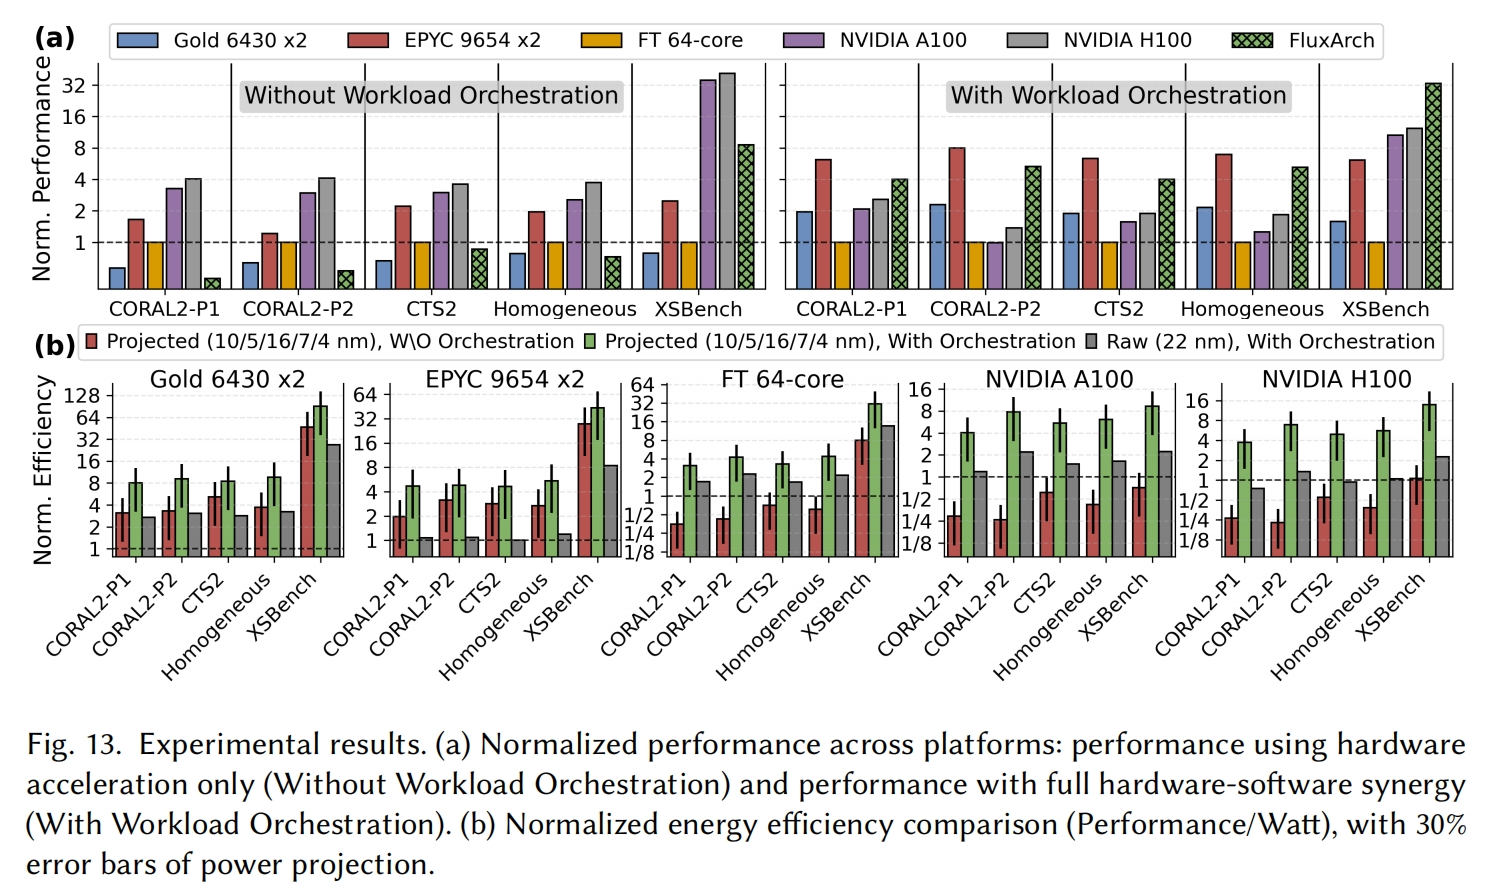
\includegraphics[width=0.9\textwidth]{figures/O-fig13.png}}
\end{figure}
\end{minipage}\par\medskip

\par\noindent\begin{minipage}{\linewidth}
\excerptlabel{Revised (Figure~13, page 16):}\par
% Revised manuscript: Figure 13
\begin{figure}[H]
  \centering
  \fbox{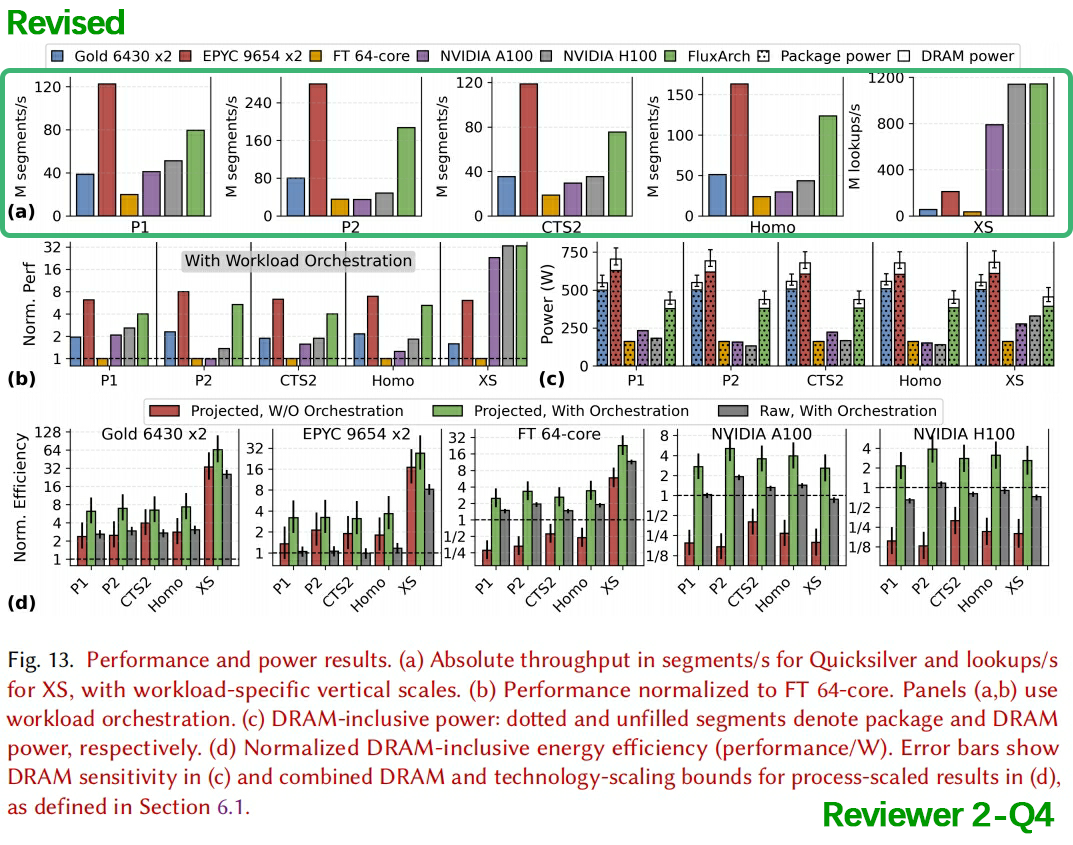
\includegraphics[width=0.9\textwidth]{news/R2-Q4-fig13.png}}
\end{figure}
\end{minipage}\par\medskip

\item \textbf{Language revision.} We carefully reviewed the language throughout the manuscript. Specifically, we corrected spelling and typographical errors, fixed grammatical issues, revised awkward sentence structures, and rephrased passages to improve clarity, fluency, and readability.

For example, in the caption of \textbf{Figure~19} in \textbf{Section 6.7}, we condensed the original three-sentence description into: ``Inter-core latency; right-side triangles denote averages, and steps mark CCD, cluster, tile, and socket boundaries.'' This replaces verbose wording such as ``The latency curve exhibits a step-like profile reflecting architectural hierarchy boundaries'' with the more direct ``steps mark CCD, cluster, tile, and socket boundaries,'' while retaining the explanation of the plotted markers and hierarchy boundaries.

\par\noindent\begin{minipage}{\linewidth}
\excerptlabel{Original (Figure~18, page 18):}\par
% Original manuscript: Figure 18
\begin{figure}[H]
  \centering
  \fbox{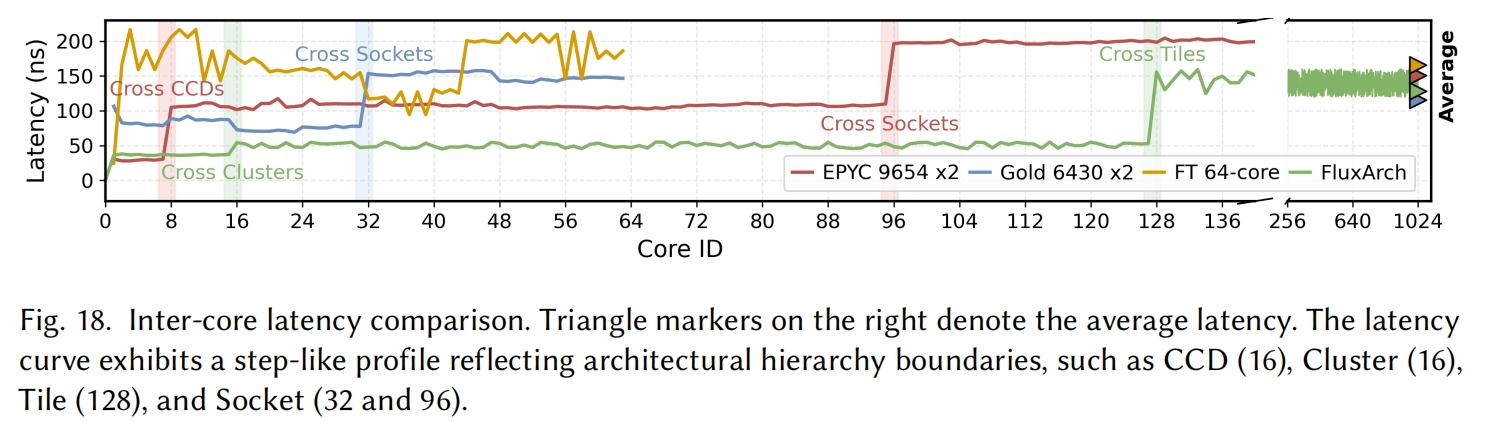
\includegraphics[width=0.9\textwidth]{figures/O-fig18.png}}
\end{figure}
\end{minipage}\par\medskip

\par\noindent\begin{minipage}{\linewidth}
\excerptlabel{Revised (Figure~19, page 21):}\par
% Revised manuscript: Figure 19
\begin{figure}[H]
  \centering
  \fbox{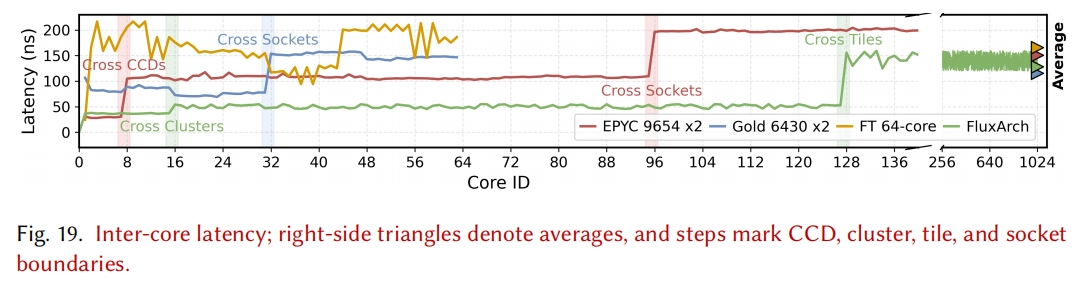
\includegraphics[width=0.9\textwidth]{news/R2-Q4-fig19.png}}
\end{figure}
\end{minipage}\par\medskip

\end{enumerate}

\subsection{Question 5}
\begin{reviewcomment}
Acknowledged but not quantified: DRAM-inclusive energy (Sec. 6.1 excludes it); whether the working set fits in 4 MB L2 --- which contradicts Fig. 3(e); load imbalance on non-uniform inputs (Sec. 7). Absent: inter-tile MPI transport and Death-Respawn cost; the MMIO programming/porting interface; absolute throughput; model validation against silicon.
\end{reviewcomment}
We sincerely thank you for your helpful and constructive suggestion. Because this comment collects eight distinct issues, we address them separately.
\begin{enumerate}[label=(\arabic*)]
\setlength{\emergencystretch}{1em}
\item \textbf{DRAM-inclusive energy.} The energy comparison now includes main-memory power rather than using an on-chip-only boundary. We added consistent accounting for co-packaged memory and off-package DDR5 plus a $0.5\times$--$2\times$ sensitivity analysis. The conservative process-scaled advantage remains above unity.

\revisionlocation{The memory-power accounting boundary and DRAM sensitivity analysis are clarified in \textbf{Section 6.1}.}

\excerptlabel{Revised (Section 6.1, page 14):}\par
\begin{manuscriptexcerpt}
\redsentence{We report DRAM-inclusive system power and energy.} \redsentence{Package power includes cores, caches, NoCs, and integrated memory controllers; for \ft, \ampare, and \hopper, the main memory is co-packaged (DDR4 or HBM) and is consequently covered by platform-level package/device telemetry.} \redsentence{In contrast, the DDR5 DIMMs of \intel\ and \amd, and the DDR5 channels assumed for \name, are physically off-package and are not covered by package-power readings.} \redsentence{We therefore add a separately modeled DRAM component to these platforms, avoiding asymmetric accounting that would include HBM/DDR4 power for the co-packaged-memory platforms but omit DDR5 power for the other platforms.}
\end{manuscriptexcerpt}

\par\noindent\begin{minipage}{\linewidth}
\revisionlocation{The resulting energy-efficiency comparison is updated in \textbf{Section 6.2}.

The DRAM-inclusive power and energy-efficiency plots are updated in \textbf{Figure~13(c,d)}. Panel (c) is newly added; panel (d) revises the original energy-efficiency plot.}

\excerptlabel{Revised (Figure~13, page 16):}\par
% Revised manuscript: Figure 13
\begin{figure}[H]
  \centering
  \fbox{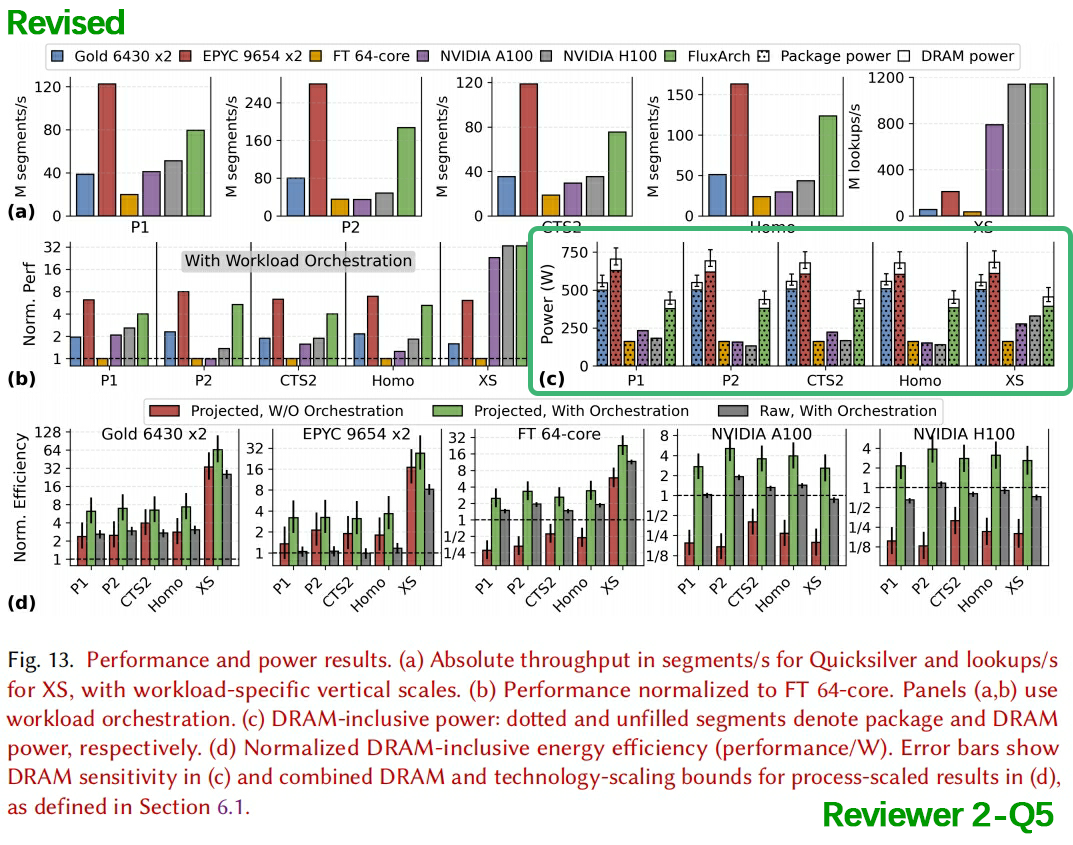
\includegraphics[width=0.9\textwidth]{news/R2-Q5-fig13.png}}
\end{figure}
\end{minipage}\par\medskip

\item \textbf{L2 working-set residency.} Our affinity mechanism provides partial shared-L2 reuse rather than universal full-working-set residency. We corrected the claim and added database-capacity and memory-traffic measurements. The 241-MiB XSBench database is about $60.25\times$ larger than the 4-MiB L2, confirming that its benefit cannot be attributed to complete residency.

\revisionlocation{The affinity mechanism is clarified in \textbf{Section 5.2} as partial shared-L2 reuse rather than full database residency.}

\excerptlabel{Revised (Section 5.2, pages 11--12):}\par
\begin{manuscriptexcerpt}
\redsentence{Shared-Database Reuse within an LLC Domain: Threads belonging to the same MPI process access a common read-mostly physics database.} \redsentence{Binding these threads to cores sharing the cluster-local 4~MB L2 allows a cache line fetched by one thread to be reused by other threads in the process.} \redsentence{This optimization does not require the complete database or working set to reside in L2.} \redsentence{Instead, the shared L2 retains a capacity-limited subset of recently accessed cache lines, reducing rather than eliminating DRAM accesses.} \redsentence{Each process places its database replica in its local NUMA memory domain, avoiding remote-memory accesses when an L2 miss occurs.}
\end{manuscriptexcerpt}

\par\noindent\begin{minipage}{\linewidth}
\revisionlocation{The memory-behavior analysis is added in \textbf{Section 6.5}.

The supporting database-capacity, L2-hit-rate, and DRAM-traffic measurements are added in \textbf{Table~6(a)}.}

\excerptlabel{Added (Table~6(a), page 18):}\par
% Revised manuscript: Table 6(a)
\begin{figure}[H]
  \centering
  \fbox{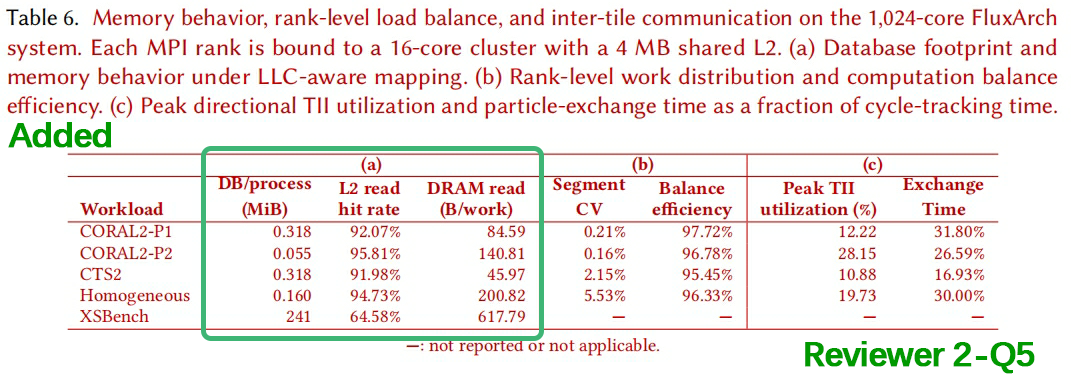
\includegraphics[width=0.9\textwidth]{news/R2-Q5-tab6a.png}}
\end{figure}
\end{minipage}\par\medskip

\item \textbf{Load imbalance.} Static spatial decomposition can create unequal stochastic work, so we added measurements across all 64 cluster-bound MPI ranks. Kernel-time CV is 1.17\%--2.01\%, balance efficiency is 95.45\%--97.72\%, and the estimated computation-side tail loss is at most 4.55\% for the evaluated inputs. These results indicate that static affinity and spatial decomposition maintain balanced computation across clusters for the evaluated workloads at 1,024 cores, with limited computation-side loss from load imbalance. More extreme inputs remain a limitation.

\revisionlocation{The rank-level load-balance evaluation and estimated computation-side tail loss are added in \textbf{Section 6.5}.}

\excerptlabel{Added (Section 6.5, pages 18--19):}\par
\begin{manuscriptexcerpt}
\redsentence{\textbf{Load Balance}.} \redsentence{Table~6(b) quantifies the concern that static affinity and spatial decomposition may assign unequal work to clusters.} \redsentence{We record completed segments and accumulated tracking-kernel time separately for all 64 ranks.} \redsentence{Segment-count CV ranges from 0.16\% to 5.53\%; because stochastic segments can follow different paths and incur different costs, count variation does not translate proportionally into execution-time variation.} \redsentence{Kernel-time CV remains 1.17\%--2.01\%.} \redsentence{We define balance efficiency as the mean rank-level kernel time divided by the maximum rank-level kernel time, since the slowest rank determines the computation tail.} \redsentence{The resulting efficiency is 95.45\%--97.72\%, corresponding to an estimated computation-side tail loss of at most 4.55\%.} \redsentence{These results indicate that static affinity and spatial decomposition maintain balanced computation across clusters for the evaluated workloads at 1,024 cores, with limited computation-side loss from load imbalance.}
\end{manuscriptexcerpt}

\par\noindent\begin{minipage}{\linewidth}
\revisionlocation{The segment-count variation and balance efficiency are reported in \textbf{Table~6(b)}.}

\excerptlabel{Added (Table~6(b), page 18):}\par
% Revised manuscript: Table 6(b)
\begin{figure}[H]
  \centering
  \fbox{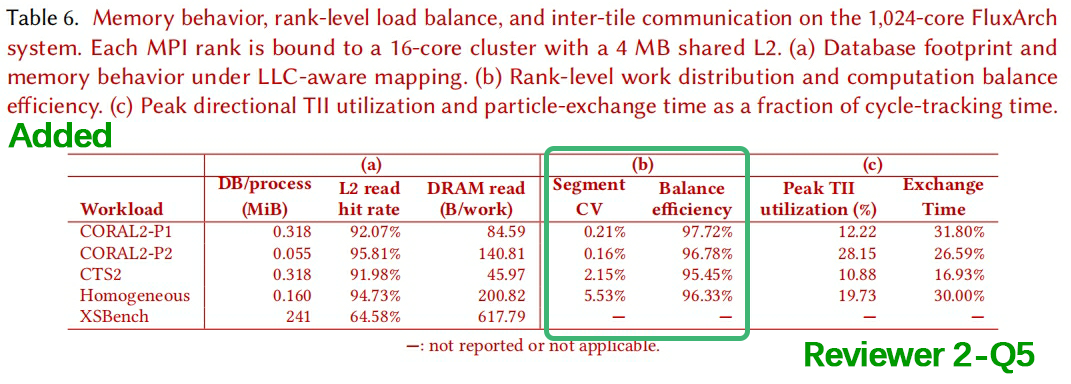
\includegraphics[width=0.9\textwidth]{news/R2-Q5-tab6b.png}}
\end{figure}
\end{minipage}\par\medskip

\item \textbf{Inter-tile MPI transport.} Inter-tile MPI transport is explicitly modeled rather than implemented as zero-cost functional communication. We added the complete path through the guest network stack, IGbE endpoints, and \texttt{DistEtherLink} TIIs and measured traffic at every interface. The busiest direction uses 10.88\%--28.15\% of the modeled 1-Gb/s capacity, with only 0.50\%--2.42\% traffic CV across TIIs.

\revisionlocation{The guest-network, IGbE, and TII transport path is specified in \textbf{Section 6.1}.}

\excerptlabel{Added (Section 6.1, page 13):}\par
\begin{manuscriptexcerpt}
\redsentence{\textbf{Inter-Tile Communication Modeling}.} \redsentence{The eight Compute Tiles are connected to the Switch Tile through eight bidirectional Tile Interconnection Interfaces (TIIs).} \redsentence{In distributed full-system gem5, each TII is modeled using a \texttt{DistEtherLink} and an IGbE endpoint, with the directional 1-Gb/s capacity in Table~1 and the modeled inter-tile latency.} \redsentence{MPI messages traverse the guest network stack and these modeled links and are therefore subject to software protocol processing, packetization, link serialization, and inter-tile latency rather than zero-cost functional communication.} \redsentence{We use the Ethernet-device counters to measure transmitted bytes and directional utilization at every TII.} \redsentence{Quicksilver's cycle-tracking timers separately measure end-to-end particle-exchange time, including buffer handling, MPI communication and waiting, and receive-side particle management.}
\end{manuscriptexcerpt}

\revisionlocation{The measured inter-tile traffic and link-utilization results are analyzed in \textbf{Section 6.7}.}

\excerptlabel{Added (Section 6.7, page 21):}\par
\begin{manuscriptexcerpt}
\redsentence{\textbf{Inter-Tile Communication Cost}.} \redsentence{Table~6(c) reports peak directional TII utilization and the particle-exchange share of cycle-tracking time.} \redsentence{Across CORAL2-P1, CORAL2-P2, CTS2 and Homogeneous, \name\ injects 1.37--1.46 bytes of inter-tile traffic per completed segment.} \redsentence{The busiest directional TII reaches only 10.88\%--28.15\% of its modeled 1-Gb/s capacity.} \redsentence{Bidirectional link traffic is also well balanced: its coefficient of variation across the eight TIIs is 0.50\%--2.42\%.} \redsentence{Thus, the communication-driven spatial mapping avoids TII hotspots, and the evaluated links remain below saturation.}
\end{manuscriptexcerpt}

\par\noindent\begin{minipage}{\linewidth}
\revisionlocation{The peak directional TII utilization and particle-exchange share are reported in \textbf{Table~6(c)}.}

\excerptlabel{Added (Table~6(c), page 18):}\par
% Revised manuscript: Table 6(c)
\begin{figure}[H]
  \centering
  \fbox{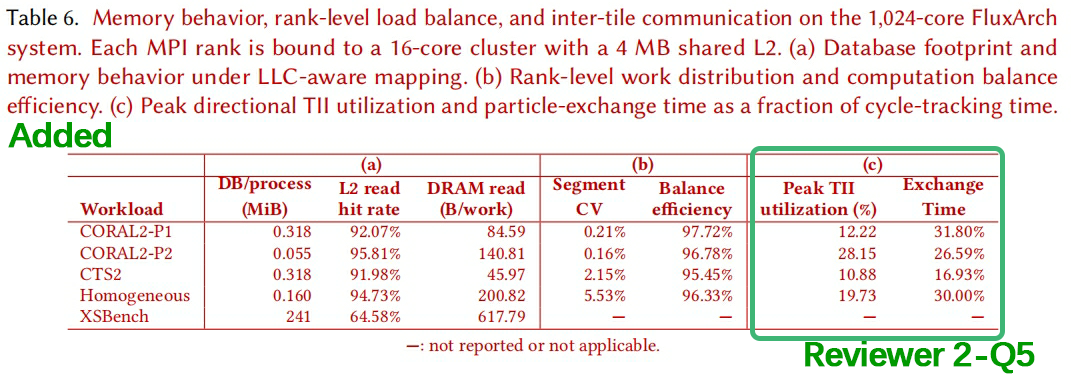
\includegraphics[width=0.9\textwidth]{news/R2-Q5-tab6c.png}}
\end{figure}
\end{minipage}\par\medskip

\item \textbf{Death-Respawn cost.} Death-Respawn and particle exchange are included in the evaluated execution path. We added an end-to-end timer covering send-buffer handling, MPI communication and waiting, receive-side particle management, and termination-related communication. This phase accounts for 16.93\%--31.80\% of cycle-tracking time, showing that it is material even though the modeled TIIs are not saturated.

\revisionlocation{The end-to-end particle-exchange measurement boundary and its distinction from pure link-transfer time are clarified in \textbf{Section 6.7}.}

\excerptlabel{Added (Section 6.7, page 21):}\par
\begin{manuscriptexcerpt}
\redsentence{Particle exchange nevertheless accounts for 16.93\%--31.80\% of cycle-tracking time.} \redsentence{This end-to-end phase includes send-buffer handling, MPI communication and waiting, receive-side particle management, and termination-related communication; it should therefore not be interpreted as pure link-transfer time.} \redsentence{Together, the measurements show that particle exchange has a measurable execution cost, but that cost cannot be attributed to saturation of the modeled TII bandwidth.}
\end{manuscriptexcerpt}
\par\noindent\begin{minipage}{\linewidth}
\revisionlocation{The particle-exchange share of cycle-tracking time is reported in \textbf{Table~6(c)}.}

\excerptlabel{Added (Table~6(c), page 18):}\par
% Revised manuscript: Table 6(c)
\begin{figure}[H]
  \centering
  \fbox{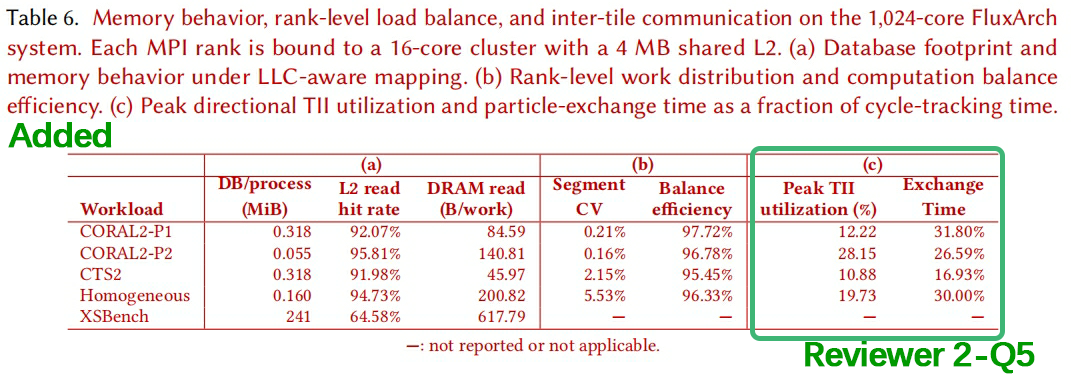
\includegraphics[width=0.9\textwidth]{news/R2-Q5-tab6c.png}}
\end{figure}
\end{minipage}\par\medskip

\item \textbf{MMIO programming and porting interface.} Each Engine is directly attached to its core's execute stage, as shown in \textbf{Figure~7}. Its MMIO interface addresses core-local registers, avoiding the interconnect traversal associated with remote MMIO peripherals. Ordinary loads and stores access the 64-bit register map, so the interface requires neither an ISA extension nor compiler modification. We clarified this local connection and added the complete operand order, launch sequence, completion protocol, and software-porting boundary in \textbf{Section 4.2} and added \textbf{Table~2(a)}. As described in \textbf{Section 6.4}, the evaluated execution path still includes the MMIO instructions, Engine synchronization, and Engine execution latency.

\revisionlocation{The core-local Engine connection, launch/completion protocol, and software-porting requirements are clarified in \textbf{Section 4.2}.}

\excerptlabel{Revised (Section 4.2, page 10):}\par
\begin{manuscriptexcerpt}
\redsentence{\textbf{Control and Programming Interface}.} \redsentence{As shown in Fig.~7, each \name\ Engine is directly attached to its core's execute stage.} \redsentence{Its memory-mapped interface provides software access to core-local registers, avoiding the interconnect traversal associated with remote MMIO peripherals.} \redsentence{The Control Unit maintains the iteration bounds and drives the nested loops in the FSM.} \redsentence{Through the 64-bit MMIO interface in Table~2(a), the host supplies the loop bounds; an accepted Control/Status write resets the internal counters and launches execution.} \redsentence{The host then streams operands and retrieves the results after \texttt{out\_valid} indicates completion.}

\redsentence{The interface is ISA-agnostic: the CPU performs database lookup in software, writes the resulting operands using ordinary stores, and reads the two final results using ordinary loads.} \redsentence{Porting therefore replaces only the stable software kernel with an MMIO wrapper; it requires neither ISA extensions nor changes to the compiler, particle representation, database layout, or MPI+OpenMP orchestration.}
\end{manuscriptexcerpt}

\par\noindent\begin{minipage}{\linewidth}
\revisionlocation{The operand order and software-visible register map are added in \textbf{Table~2(a)}.}

\excerptlabel{Added (Table~2(a), page 10):}\par
% Revised manuscript: Table 2(a)
\begin{figure}[H]
  \centering
  \fbox{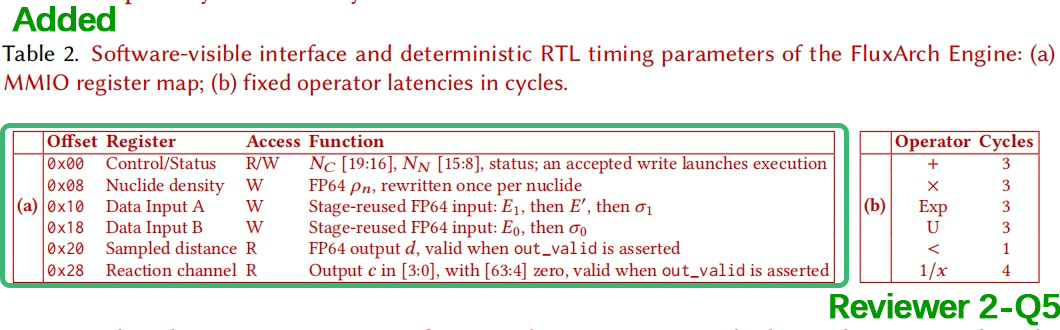
\includegraphics[width=0.9\textwidth]{news/R2-Q5-tab2a.png}}
\end{figure}
\end{minipage}\par\medskip

\item \textbf{Absolute throughput.} We supplemented normalized speedup with absolute throughput for every workload and platform. The revised results use segments/s for Quicksilver and lookups/s for XSBench and derive the normalized values from the same measurements. \name\ reaches 75.33--186.70 million segments/s across the Quicksilver inputs and 1.143 billion XSBench lookups/s.

\revisionlocation{The absolute throughput values and the units for Quicksilver and XSBench are specified in \textbf{Section 6.2}.}

\excerptlabel{Original (Section 6.2, page 14):}\par
\begin{manuscriptexcerpt}
\graysentence{\textbf{Performance Impact}.} \graysentence{Fig.~13(a) presents the performance of platforms across five benchmarks, normalized to the \ft.} \graysentence{The results underscore a cooperation between the domain-specific architecture and the synergistic workload orchestration.}

\graysentence{Without the synergistic workload orchestration, \name\ offers little to no advantage over CPUs and GPUs, ranging from 0.17$\times$ (vs. \hopper) to 1.54$\times$ (vs. \intel), due to severe interconnect contention and non-local memory traffic.} \graysentence{Crucially, enabling the workload orchestration unlocks the full potential of \name\ to surpass all of the platforms, boosting the geometric mean speedup from \textbf{1.02}$\boldsymbol{\times}$ (vs. \amd) to \textbf{6.83}$\boldsymbol{\times}$ (vs. \ft).}
\end{manuscriptexcerpt}

\excerptlabel{Revised (Section 6.2, page 15):}\par
\begin{manuscriptexcerpt}
\redsentence{\textbf{Performance Impact}.} \redsentence{Fig.~13(a,b) reports absolute throughput and values normalized to \ft.} \redsentence{\name\ achieves 79.33, 186.70, 75.33, and 123.50 million segments/s for P1, P2, CTS2, and Homo, respectively, and 1.143 billion XS lookups/s, yielding geometric-mean speedups from \textbf{1.02}$\boldsymbol{\times}$ over \amd\ to \textbf{6.83}$\boldsymbol{\times}$ over \ft.}
\end{manuscriptexcerpt}

\par\noindent\begin{minipage}{\linewidth}
\revisionlocation{The per-platform absolute throughput and corresponding normalized results are presented in \textbf{Figure~13(a,b)}. Panel (a) is newly added; panel (b) revises the original normalized-performance plot.}

\excerptlabel{Revised (Figure~13, page 16):}\par
% Revised manuscript: Figure 13
\begin{figure}[H]
  \centering
  \fbox{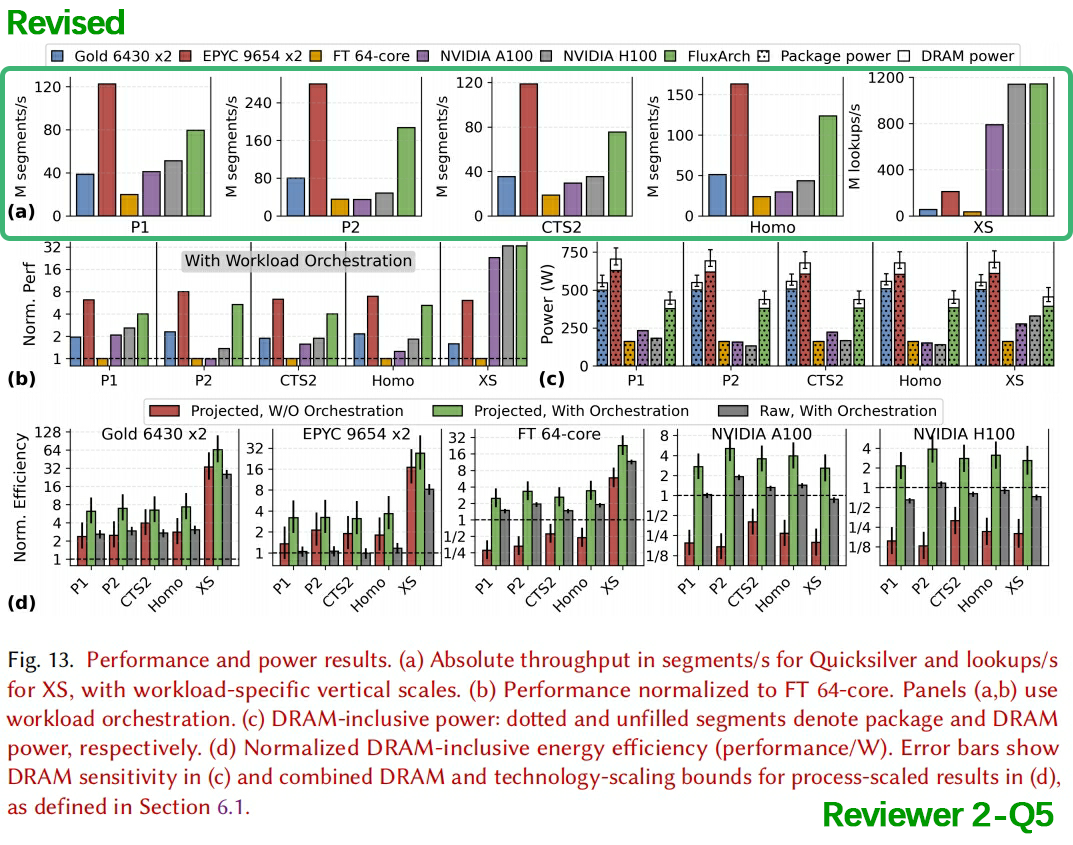
\includegraphics[width=0.9\textwidth]{news/R2-Q5-fig13a.png}}
\end{figure}
\end{minipage}\par\medskip

\item \textbf{Model validation against silicon.} As detailed in our response to \textbf{R2-Q1, item (2)}, six RK3562 silicon comparisons calibrate the core and cache/DRAM paths, with 6.7\% mean and 13.5\% maximum absolute percentage errors. The RTL-derived Engine timing establishes implementation traceability, not independent silicon validation; the complete 1,024-core hierarchy remains evaluated through calibrated simulation rather than a fabricated prototype. The supporting manuscript excerpts and calibration results are provided in that response. The distinction between native baseline measurements and simulated \name\ results is documented in \textbf{R2-Q1, item (1)}.\looseness=-1

\end{enumerate}
